\documentclass{standalone}
\usepackage{tikz}
\usetikzlibrary{patterns, positioning}


\begin{document}
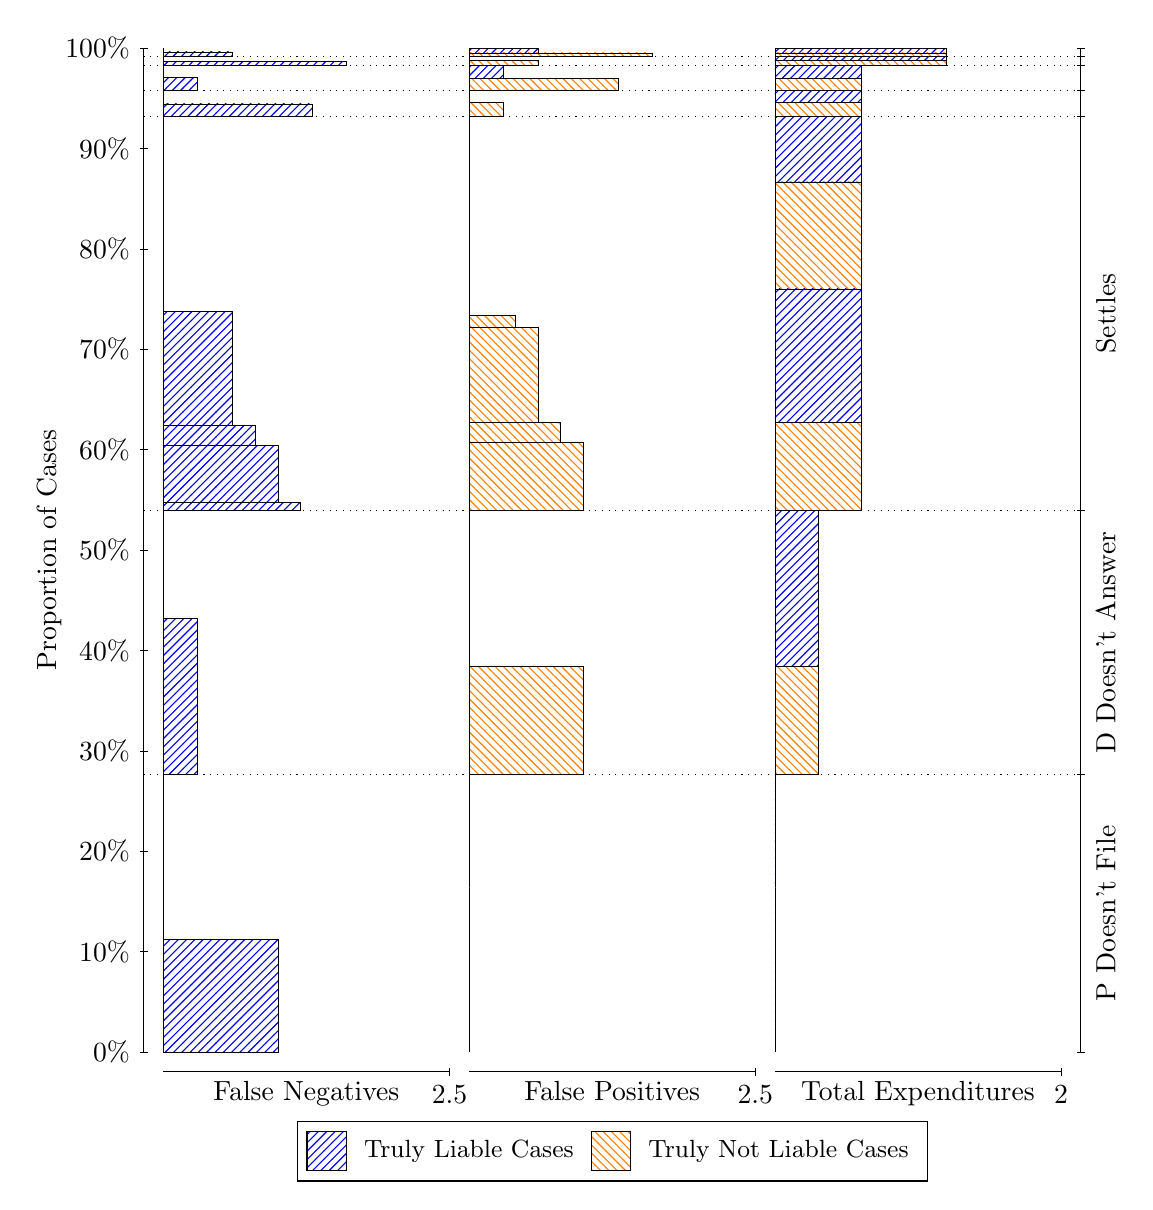
\begin{tikzpicture}
\draw[black, very thin] (1.5,1.75) -- (1.5,14.5);
\node[rotate=90, text=black, anchor=center] at (0.3, 8.125) {Proportion of Cases};
\draw[black, very thin] (1.45,1.75) -- (1.55,1.75);
\node[text=black, anchor=east] at (1.45, 1.75) {0\%};
\draw[black, very thin] (1.45,3.025) -- (1.55,3.025);
\node[text=black, anchor=east] at (1.45, 3.025) {10\%};
\draw[black, very thin] (1.45,4.3) -- (1.55,4.3);
\node[text=black, anchor=east] at (1.45, 4.3) {20\%};
\draw[black, very thin] (1.45,5.575) -- (1.55,5.575);
\node[text=black, anchor=east] at (1.45, 5.575) {30\%};
\draw[black, very thin] (1.45,6.85) -- (1.55,6.85);
\node[text=black, anchor=east] at (1.45, 6.85) {40\%};
\draw[black, very thin] (1.45,8.125) -- (1.55,8.125);
\node[text=black, anchor=east] at (1.45, 8.125) {50\%};
\draw[black, very thin] (1.45,9.4) -- (1.55,9.4);
\node[text=black, anchor=east] at (1.45, 9.4) {60\%};
\draw[black, very thin] (1.45,10.675) -- (1.55,10.675);
\node[text=black, anchor=east] at (1.45, 10.675) {70\%};
\draw[black, very thin] (1.45,11.95) -- (1.55,11.95);
\node[text=black, anchor=east] at (1.45, 11.95) {80\%};
\draw[black, very thin] (1.45,13.225) -- (1.55,13.225);
\node[text=black, anchor=east] at (1.45, 13.225) {90\%};
\draw[black, very thin] (1.45,14.5) -- (1.55,14.5);
\node[text=black, anchor=east] at (1.45, 14.5) {100\%};

\draw[black, very thin] (13.4,1.75) -- (13.4,14.5);
\draw[black, very thin] (13.35,1.75) -- (13.45,1.75);
\node[anchor=west] at (13.35, 1.75) {};
\draw[black, very thin] (13.35,5.2722) -- (13.45,5.2722);
\node[anchor=west] at (13.35, 5.2722) {};
\draw[black, very thin] (13.35,8.625) -- (13.45,8.625);
\node[anchor=west] at (13.35, 8.625) {};
\draw[black, very thin] (13.35,13.632) -- (13.45,13.632);
\node[anchor=west] at (13.35, 13.632) {};
\draw[black, very thin] (13.35,13.966) -- (13.45,13.966);
\node[anchor=west] at (13.35, 13.966) {};
\draw[black, very thin] (13.35,14.28) -- (13.45,14.28);
\node[anchor=west] at (13.35, 14.28) {};
\draw[black, very thin] (13.35,14.39) -- (13.45,14.39);
\node[anchor=west] at (13.35, 14.39) {};
\draw[black, very thin] (13.35,14.5) -- (13.45,14.5);
\node[anchor=west] at (13.35, 14.5) {};

\draw[black, very thin, pattern color=blue, pattern=north east lines] (1.75,1.75) rectangle (3.2033,3.1818);
\draw[black, very thin, pattern color=orange, pattern=north west lines] (1.75,3.1818) rectangle (1.75,5.2722);
\draw[black, very thin, pattern color=blue, pattern=north east lines] (1.75,5.2722) rectangle (2.186,7.2551);
\draw[black, very thin, pattern color=orange, pattern=north west lines] (1.75,7.2551) rectangle (1.75,8.625);
\draw[black, very thin, pattern color=blue, pattern=north east lines] (1.75,8.625) rectangle (3.494,8.7291);
\draw[black, very thin, pattern color=blue, pattern=north east lines] (1.75,8.7291) rectangle (3.3487,8.7332);
\draw[black, very thin, pattern color=blue, pattern=north east lines] (1.75,8.7332) rectangle (3.2033,9.4571);
\draw[black, very thin, pattern color=blue, pattern=north east lines] (1.75,9.4571) rectangle (2.9127,9.7037);
\draw[black, very thin, pattern color=blue, pattern=north east lines] (1.75,9.7037) rectangle (2.622,11.155);
\draw[black, very thin, pattern color=orange, pattern=north west lines] (1.75,11.155) rectangle (1.75,13.632);
\draw[black, very thin, pattern color=blue, pattern=north east lines] (1.75,13.632) rectangle (3.6393,13.79);
\draw[black, very thin, pattern color=orange, pattern=north west lines] (1.75,13.79) rectangle (1.75,13.966);
\draw[black, very thin, pattern color=blue, pattern=north east lines] (1.75,13.966) rectangle (2.186,14.128);
\draw[black, very thin, pattern color=orange, pattern=north west lines] (1.75,14.128) rectangle (1.75,14.28);
\draw[black, very thin, pattern color=blue, pattern=north east lines] (1.75,14.28) rectangle (4.0753,14.329);
\draw[black, very thin, pattern color=orange, pattern=north west lines] (1.75,14.329) rectangle (1.75,14.39);
\draw[black, very thin, pattern color=blue, pattern=north east lines] (1.75,14.39) rectangle (2.622,14.452);
\draw[black, very thin, pattern color=orange, pattern=north west lines] (1.75,14.452) rectangle (1.75,14.5);
\draw[black, very thin, pattern color=orange, pattern=north west lines] (5.6333,1.75) rectangle (5.6333,3.8404);
\draw[black, very thin, pattern color=blue, pattern=north east lines] (5.6333,3.8404) rectangle (5.6333,5.2722);
\draw[black, very thin, pattern color=orange, pattern=north west lines] (5.6333,5.2722) rectangle (7.0867,6.6421);
\draw[black, very thin, pattern color=blue, pattern=north east lines] (5.6333,6.6421) rectangle (5.6333,8.625);
\draw[black, very thin, pattern color=orange, pattern=north west lines] (5.6333,8.625) rectangle (7.0867,9.496);
\draw[black, very thin, pattern color=orange, pattern=north west lines] (5.6333,9.496) rectangle (6.796,9.7427);
\draw[black, very thin, pattern color=orange, pattern=north west lines] (5.6333,9.7427) rectangle (6.5053,10.949);
\draw[black, very thin, pattern color=orange, pattern=north west lines] (5.6333,10.949) rectangle (6.36,10.955);
\draw[black, very thin, pattern color=orange, pattern=north west lines] (5.6333,10.955) rectangle (6.2147,11.102);
\draw[black, very thin, pattern color=blue, pattern=north east lines] (5.6333,11.102) rectangle (5.6333,13.632);
\draw[black, very thin, pattern color=orange, pattern=north west lines] (5.6333,13.632) rectangle (6.0693,13.808);
\draw[black, very thin, pattern color=blue, pattern=north east lines] (5.6333,13.808) rectangle (5.6333,13.966);
\draw[black, very thin, pattern color=orange, pattern=north west lines] (5.6333,13.966) rectangle (7.5227,14.118);
\draw[black, very thin, pattern color=blue, pattern=north east lines] (5.6333,14.118) rectangle (6.0693,14.28);
\draw[black, very thin, pattern color=orange, pattern=north west lines] (5.6333,14.28) rectangle (6.5053,14.342);
\draw[black, very thin, pattern color=blue, pattern=north east lines] (5.6333,14.342) rectangle (5.6333,14.39);
\draw[black, very thin, pattern color=orange, pattern=north west lines] (5.6333,14.39) rectangle (7.9587,14.439);
\draw[black, very thin, pattern color=blue, pattern=north east lines] (5.6333,14.439) rectangle (6.5053,14.5);
\draw[black, very thin, pattern color=orange, pattern=north west lines] (9.5167,1.75) rectangle (9.5167,3.8404);
\draw[black, very thin, pattern color=blue, pattern=north east lines] (9.5167,3.8404) rectangle (9.5167,5.2722);
\draw[black, very thin, pattern color=orange, pattern=north west lines] (9.5167,5.2722) rectangle (10.062,6.6421);
\draw[black, very thin, pattern color=blue, pattern=north east lines] (9.5167,6.6421) rectangle (10.062,8.625);
\draw[black, very thin, pattern color=orange, pattern=north west lines] (9.5167,8.625) rectangle (10.607,9.7427);
\draw[black, very thin, pattern color=blue, pattern=north east lines] (9.5167,9.7427) rectangle (10.607,11.44);
\draw[black, very thin, pattern color=orange, pattern=north west lines] (9.5167,11.44) rectangle (10.607,12.8);
\draw[black, very thin, pattern color=blue, pattern=north east lines] (9.5167,12.8) rectangle (10.607,13.632);
\draw[black, very thin, pattern color=orange, pattern=north west lines] (9.5167,13.632) rectangle (10.607,13.808);
\draw[black, very thin, pattern color=blue, pattern=north east lines] (9.5167,13.808) rectangle (10.607,13.966);
\draw[black, very thin, pattern color=orange, pattern=north west lines] (9.5167,13.966) rectangle (10.607,14.118);
\draw[black, very thin, pattern color=blue, pattern=north east lines] (9.5167,14.118) rectangle (10.607,14.28);
\draw[black, very thin, pattern color=orange, pattern=north west lines] (9.5167,14.28) rectangle (11.697,14.342);
\draw[black, very thin, pattern color=blue, pattern=north east lines] (9.5167,14.342) rectangle (11.697,14.39);
\draw[black, very thin, pattern color=orange, pattern=north west lines] (9.5167,14.39) rectangle (11.697,14.439);
\draw[black, very thin, pattern color=blue, pattern=north east lines] (9.5167,14.439) rectangle (11.697,14.5);
\draw[black, dotted] (1.5,5.2722) -- (13.4,5.2722);
\draw[black, dotted] (1.5,8.625) -- (13.4,8.625);
\draw[black, dotted] (1.5,13.632) -- (13.4,13.632);
\draw[black, dotted] (1.5,13.966) -- (13.4,13.966);
\draw[black, dotted] (1.5,14.28) -- (13.4,14.28);
\draw[black, dotted] (1.5,14.39) -- (13.4,14.39);
\draw[black, very thin] (1.75,1.5) -- (5.3833,1.5);
\node[text=black, anchor=north] at (3.5667, 1.5) {False Negatives};
\draw[black, very thin] (5.3833,1.45) -- (5.3833,1.55);
\node[text=black, anchor=north] at (5.3833, 1.45) {2.5};

\draw[black, very thin] (5.6333,1.5) -- (9.2667,1.5);
\node[text=black, anchor=north] at (7.45, 1.5) {False Positives};
\draw[black, very thin] (9.2667,1.45) -- (9.2667,1.55);
\node[text=black, anchor=north] at (9.2667, 1.45) {2.5};

\draw[black, very thin] (9.5167,1.5) -- (13.15,1.5);
\node[text=black, anchor=north] at (11.333, 1.5) {Total Expenditures};
\draw[black, very thin] (13.15,1.45) -- (13.15,1.55);
\node[text=black, anchor=north] at (13.15, 1.45) {2};

\node[text=black, centered, rotate=90] at (13.72, 3.5111) {P Doesn't File};
\node[text=black, centered, rotate=90] at (13.72, 6.9486) {D Doesn't Answer};
\node[text=black, centered, rotate=90] at (13.72, 11.128) {Settles};





\draw (7.449999999999999,1.5) node[draw=none] (baseCoordinate) {};
\begin{scope}[align=center]
        \matrix[scale=0.5, draw=black, below=0.5cm of baseCoordinate, nodes={draw}, column sep=0.1cm]{
            \node[rectangle, draw, minimum width=0.5cm, minimum height=0.5cm, pattern color=blue, pattern=north east lines] {}; &
            \node[draw=none, font=\small, text=black] (B) {Truly Liable Cases}; &
            \node[rectangle, draw, minimum width=0.5cm, minimum height=0.5cm, pattern color=orange, pattern=north west lines] {}; &
            \node[draw=none, font=\small, text=black] (B) {Truly Not Liable Cases}; \\
            };
\end{scope}

\end{tikzpicture}
\end{document}